\documentclass[UTF8,12.05pt]{ctexart}
\usepackage{graphicx}
\usepackage{geometry}
\geometry{a4paper,margin=2.8cm}
\usepackage{fancyhdr}
\usepackage{listings}
\usepackage{appendix}
\usepackage{xcolor}
\usepackage{float}
\usepackage{amsmath}
\usepackage{amssymb}
\usepackage{fancyhdr}
\pagestyle{empty}
\begin{document}
\bibliographystyle{plain}
\begin{center}
  \zihao{3}\heiti交通事故引起的车道被占用对城市交通的影响
\end{center}

\vspace{1cm}
\begin{abstract}
\zihao{-4}
车道被占用是指因交通事故、路边停车、占道施工等因素,导致车道或道路横断面通行能力在单位时间内降低的现象。由于城市道路具有交通流密度大、连续性强等特点,一条车道被占用,也可能降低路段所有车道的通行能力,即使时间短,也可能引起车辆排队,出现交通阻塞。如处理不当,甚至出现区域性拥堵。本文针对车道被占用的交通问题,构建数学模型,给出以下四个问题的解答。
\par问题一要求我们描述道路通行能力的变化情况,车道的服务水平决定道路的通行能力,当发生交通事故时通行能力会发生变化。所以问题一分成两小问来回答,(1)估算正常情况下道路的通行能力,(2)估算事故发生后道路的通行能力。首先我们用基于延误的pcu算法将混合车流的不同车型换算成标准小汽车。对于第一小问,我们先根据道路通行手册\cite{road}计算出视频中三车道双幅路的理论通行能力,在此基础上经过车道宽度,交叉口,车道数修正因数修正得到正常通行时实际通行能力为3600pcu/h。对于第二小问,我们通过观察估算法,得到有事故车辆占道时车流量的变化,用Excel绘制出图表,取最大值为发生交通事故道路的通行能力为\newline1300pcu/h。
\par针对问题二对于所占车道的不同比较实际通行能力的差异,我们首先用Excel绘制图表对占道不同的车流量时间分布进行描述,发现当被占车道车辆比例小时,道路的通行能力较大,在假定上游车流量一定的情况下,用参数回归得到实际通行能力与被占车道车辆比例关系。
\par针对问题三,我们构建了元胞传输模型(CTM)描述车辆排队长度和事故横断面实际通行能力、事故持续时间、路段上游车流量间的关系,CTM将路段分成多个等距的小段(元胞),每一个元胞有车流密度,流量等属性进行描述,元胞之间相互的影响根据LWR理论建模,CTM状态方程则以\newline Daganzo对于流量和密度关系假设的基础上建立起来,用MATLAB软件对模型进行仿真得到不同上游车流量和横断面通行能力的条件下,车辆排队长度随时间的变化。用车流波动理论对仿真结果进行解释。
\par我们用问题三的元胞传输模型对于问题四进行求解,不考虑信号灯的控制和小区路口影响时我们用MATLAB仿真得到排队长度到达上游路口的时间为12分钟,考虑信号灯和小区路口影时,我们用vissim软件进行仿真得到时间为10分钟。
\begin{flushleft}
  \textbf{关键词:}元胞运输模型;\quad车辆折算系数;\quad vissim仿真。
\end{flushleft}
\end{abstract}
\newpage
\pagestyle{plain}
\pagenumbering{arabic}
\setcounter{page}{1}
\section{\heiti\zihao{4}问题重述}
\normalsize车道被占用是指因交通事故、路边停车、占道施工等因素,导致车道或道路横断面通行能力在单位时间内降低的现象。由于城市道路具有交通流密度大、连续性强等特点,一条车道被占用,也可能降低路段所有车道的通行能力,即使时间短,也可能引起车辆排队,出现交通阻塞。如处理不当,甚至出现区域性拥堵。
\par车道被占用的情况种类繁多、复杂,正确估算车道被占用对城市道路通行能力的影响程度,将为交通管理部门正确引导车辆行驶、审批占道施工、设计道路渠化方案、设置路边停车位和设置非港湾式公交车站等提供理论依据。
视频1(附件1)和视频2(附件2)中的两个交通事故处于同一路段的同一横断面,且完全占用两条车道。请研究以下问题:
\begin{itemize}
  \item 问题1:根据视频1(附件1),描述视频中交通事故发生至撤离期间,事故所处横断面实际通行能力的变化过程。
  \item 问题2:  根据问题1所得结论,结合视频2(附件2),分析说明同一横断面交通事故所占车道不同对该横断面实际通行能力影响的差异。
  \item 问题3:  构建数学模型,分析视频1(附件1)中交通事故所影响的路段车辆排队长度与事故横断面实际通行能力、事故持续时间、路段上游车流量间的关系。
  \item 问题4:  假如视频1(附件1)中的交通事故所处横断面距离上游路口变为140米,路段下游方向需求不变,路段上游车流量为1500pcu/h,事故发生时车辆初始排队长度为零,且事故持续不撤离。请估算,从事故发生开始,经过多长时间,车辆排队长度将到达上游路口。
\end{itemize}
\section{\heiti\zihao{4}模型的假设}
\begin{enumerate}
  \item 不考虑摩托车自行车等二轮交通工具以及行人对该路段交通运行的影响;
  \item 事故发生后交通运行处在正常的道路、交通、管制以及运行质量要求的条件下;
  \item 不考虑视频以外的路段以及对向车道的影响的影响;
  \item 道路通行能力在相同的交通条件下相同;
  \item 忽视个别司机的交通行为对交通状况的影响;
  \item 每一条车道的服务水平相同。
\end{enumerate}
\section{\heiti\zihao{4}符号说明}
\begin{table}[H]
  \centering
  \begin{tabular}{|c| c| c|}
  \hline
  % after \\: \hline or \cline{col1-col2} \cline{col3-col4} ...
  序号&关键符号&符号说明 \\ \hline
  1&$\large D\_PCU$&车型i基于延误的车辆折算系数 \\      \hline
  2&$\large \Delta$&车型i进入车流后引起的附加延误量 \\ \hline
  3&$\large d_{0}$&在纯小汽车交通环境下,小汽车的平均延误 \\ \hline
  4&$\large C_{0}$&一条车道的道路的理论通行能力 \\ \hline
  5&$\large L_{0}$&——停车时车辆安全车间距(m) \\ \hline
  6&$\large L_{1}$&行驶速度\\ \hline
  7&$\large I$&与车重、路面阻力系数、粘着系数及坡度有关的系数\\ \hline
  8&$\large U$&驾驶员在反应时间内车辆的行驶距离\\ \hline
  9&$\large n$&车道数\\ \hline
  10&$\large C$&n条车道的理论通行能力\\ \hline
  11&$\large \alpha$&车道利用系数\\ \hline
  12&$\large \eta$&车辆在交叉口手影响的概率\\ \hline
  13&$\large T$&事故的持续时间 \\ \hline
  14&$\large q_{i}(k)$&第k个时段元胞i上的流入率 \\ \hline
  15&$\large \rho_{i}(k)$&第k个时段元胞i上的车流密度\\ \hline
  16&$\large x$&空间位置 \\ \hline
  17&$\large v_{f}$&自由流速度\\ \hline
  18&$\large \omega$&交通拥挤时车流波反向传播速度 \\ \hline
  19&$\large q_{i,max}(k)$&第k个时段元胞i的最大流率 \\ \hline
  20&$\large n_{i}(k)$&第k个时段元胞i上的车辆数 \\ \hline
  21&$\large y_{i}(k)$&第k个时段元胞i上的流入量 \\ \hline
  22&$\large Q_{i}(k)$&第k个时段元胞i上的最大流入量 \\ \hline
  23&$\large N_{i}(k)$&第k个时段元胞i上的最大承载能力 \\ \hline
  23&$\large s_{f}$&饱和流量 \\ \hline
  24&$\large L_{j}$&排队长度 \\ \hline
\end{tabular}
\end{table}
\newpage
\section{\heiti\zihao{4}问题一的分析和解答}
\subsection{问题分析}
问题一要求描述视频1中交通事故发生至撤离期间,事故所处横断面实际通行能力的变化过程。
\par道路通行能力是指道路设施所能疏导交通流的能力。即在一定的时段和正常的道路、交通、管制及运行质量要求下,道路设施通过交通流质点的能力。道路通行能力的传统计算方法是根据一条车道的理论通行能力,经过相关影响通行能力的因素修正而得到实际通行能力,即在理论通行能力基础上考虑相关因素的折减,如车道宽度影响修正系数、自行车影响修正系数、交叉口影响修正系数、车道数修正系数等,所以道路通行能力与车道数、横断面形式密切相关,而与车流的速度和密度无关,所以题目中要求我们描述实际通行能力的变化过程,指的应是从正常情况下变为有事故车辆占道道路通行能力的变化。
\par通过对视频1的观察可得,城市道路的横断面形式为双幅式,由中间一条分隔带将车行道分为单向行驶的两条车行道,每条车行道由三条车道组成,可避免对向行驶车辆的干扰,但机动车和非机动车仍然混合行驶。在视频中行驶在双幅路上的非机动车较少,所以可以忽略其影响\cite{U49}.
\par在发生事故前,路段的通行能力为单向三车道的通行能力。三车道内侧事故发生后,由于事故车辆占道,致使通过事故瓶颈路段车道数减少,此时整个事故路段的通行能力实质上取决于事故瓶颈路段的通行能力\cite{10004}。
\par首先对视频中车流数据进行采集,双幅路车辆类型混杂,各种车型间的动力性能相差悬殊,造成不同车型在道路上行驶时所占用的时间和空间大不相同。在进行通行能力研究时不同车型的交通量之间没有可比性,为此需将不同车型的交通量乘以车辆换算系数换成某一标准车型(小汽车)的交通量(PCU),以量化不同车型的车辆对通行能力的影响\cite{1006}。
\par大型客车在遇到事故地点变向时,消耗的时空资源与事故发生前直行时消耗的时空资源相比明显不相同。在拥挤或者车辆强烈的相互作用的情况下,需要占用更多的道路空间,所以在这两种不同的情况下,车辆变换系数也是不同,这里采用延误的PCU算法,基于延误的算法可以确保混合交通流和等价的纯小汽车流具有相同的总延误量\cite{U492}。
\par视频中缺乏描述正常道路条件下通行能力的数据,我们根据道路的实际情况,从道路通行能力的定义出发得到该路段正常通行时通行能力定量的衡量。
\par我们用观测估算法估算事故发生后道路的通行能力,首先我们要统计单位时间内通过事故截面的流量。因为上游交叉口信号灯第一相位和第二相位的时间皆为30s,考虑到上游信号灯的变化对该路段车流量的影响比较显著,所以我们以30s为单位时间统计通过事故所处横断面的标准汽车当量,通过Excel绘制车流量的时间分布。主要关注图像中的极大值。

\subsection{模型建立和求解}
\subsubsection{基于延误的车辆换算}
延误计算方法的提出是基于一下概念,当车流中存在存在车型i而造成的延误附加值与由于车型i造成的通行能力的减少效果有相关性。基于延误的PCE算法定义为由车型i引起的延误与纯小客车流中小客车的延误的比值,计算方程如下式
$$D\_PCU=1+\frac{\Delta_{i}}{d_{0}}$$
其中 $D\_PCU$——车型i基于延误的车辆折算系数;
\par$\Delta_{i}$——车型i进入车流后引起的附加延误量;
\par$d_{0}$——在纯小汽车交通环境下,小汽车的平均延误。
\par观察视频中多组不同类型的交通流通过某一截面的时间,例如:
\begin{itemize}
  \item 16:40:21-16:40:27 6辆小汽车通过该路段某一截面;
  \item 16:40:32-16:40:40 5辆小汽车和一辆大型客车通过某一截面。
\end{itemize}
得到大型车辆的大致换算系数如下表:
\begin{table}[H]
  \centering
  \caption{大型车辆换算系数}
  \begin{tabular}{|c|c|c|}
    \hline
    % after \\: \hline or \cline{col1-col2} \cline{col3-col4} ...
    交通路况 & 事故前 & 事故后 \\ \hline
    换算关系 & 1.5 & 2 \\
    \hline
  \end{tabular}
\end{table}
\subsubsection{正常情况下道路通行能力}
对于正常运交通条件下道路的通行能力,视频中没有足够的信息对其进行描述,我们从道路通行能力的定义出发得到该路段通行能力定量的衡量。理论通行能力是指在理想的道路和交通条件下,车辆以连续车流形式通过时的通行能力,其计算公式为
$$C_{0}=\frac{1000V}{L}$$
\par式中 $C_{0}$——一条车道的道路的理论通行能力(辆/h);
\par$V$——行驶速度(km/h);
\par$L$——连续车流的车头间距(m)。
\par连续车流条件下的车头间距L,可采用下式计算:
$$L=L_{0}+L_{1}+U+I\times V^{2}$$
\par式中:$L_{0}$——停车时车辆安全车间距(m);
\par$L_{1}$——车辆的车身长度(m);
\par$V$——行驶速度(km/h);
\par$I$——与车重、路面阻力系数、粘着系数及坡度有关的系数;
\par$U$——驾驶员在反应时间内车辆行驶的距离(m).$U=VT$,$T=1.2s$左右。
\par在通常的城市道路设计规范内(坡度$\leqslant |4\%|$),其中I值近似为0.054,取$L_{0}=2m$,小汽车的车身长度$L_{1}=5m$,则一条车道的理论通行能力如下表所示。
\begin{table}[H]
  \centering
  \caption{一条车道的理论通行能力}
  \begin{tabular}{c| c| c|c|c|c}
  \hline
  % after \\: \hline or \cline{col1-col2} \cline{col3-col4} ...
  v(km/h)&20&30&40&50&60 \\ \hline
  $C_{0}(pcu/h)$&1380&1550&1640&1690&1730 \\ \hline
\end{tabular}
\end{table}
由于基本通行能力计算式不考虑道路和交通条件的影响,因此多车道的基本通行能力可按下式计算:
$$C=n\times C_{0}$$
\par式中:n——车道数;
\par C——n条车道的基本通行能力;
\par $C_{0}$——一条车道的基本通行能力。
\newline
\par上述公式计算所得的基本通行能力的值是理想条件下的交通量,事实上各路段上行驶的车辆道路交通环境的不同而有所变化。实际通行能力是指考虑到道路和交通条件的影响,并对基本通行能力进行修正后得到的通行能力,实际上是指道路所能承担的最大交通量。影响路道可能通行能力的影响因素有:车道数、交叉口、车道宽度等。下面介绍下这些影响因素。
\paragraph{多车道对路段通行能力的影响}
在多车道的情况下,通向行驶的车辆由于超车、停车等原因影响另一条车道上的车辆行驶,从而影响其通行能力。一般越靠近道路中心线的车道,对其影响最小,因此,在无分隔带的同向行驶的车道上,靠近到道路中心线的车道通行能力最大;靠近侧石道,其通行能力最小。其影响用折减系数用条$\alpha_{\text{条}}$ 表示,其值可根据车道的利用系数确定\cite{chedao}我国通常采用的车道利用系数如下表所示
\begin{table}[H]
  \centering
  \caption{我国常用的车道利用系数}
  \begin{tabular}{|c|c|c|c|c|}
    \hline
    % after \\: \hline or \cline{col1-col2} \cline{col3-col4} ...
    车道 & 第一车道 & 第二车道 & 第三车道 & 第四车道 \\ \hline
    车道利用系数 & 1.0 & $0.8\sim0.89$ & $0.65\sim0.70$ & $0.5\sim0.65$ \\
    \hline
  \end{tabular}
\end{table}
\par根据国内外研究结果,在具体规划是,可采用下表的车道修正系数。
\begin{table}[H]
  \centering
  \caption{车道数折减系数采用值$\alpha$}
  \begin{tabular}{|c|c|c|c|c|}
    \hline
    % after \\: \hline or \cline{col1-col2} \cline{col3-col4} ...
    车道数 & 一条车道 & 二条车道 & 三条车道 & 四条车道 \\ \hline
    车道数折减系数$\alpha$ & 1.0 & 1.87 & 2.65 & 3.2 \\
    \hline
  \end{tabular}
\end{table}
\paragraph{交叉口对路段通行能力的影响}
路段中小区的出入口形成了两个交叉口,,这些交叉口对路段通行能力的影响较大。车辆通过交叉口时,有一定概率需要减速通行或者停车让行,所以当车辆通过交叉口时,实际的行程时间比没有交叉口的路段的行程时间要多,其实际平均速度也大大降低,通行能力下降。
\par交叉口对路段通行能力的影响,用交叉口通行能力折减系数$\alpha_{\text{交}}$来表示,
$$\alpha_{\text{交}}=\frac{\frac{l}{v}}{\frac{l}{v}+\eta\times(\frac{v}{2a}+\frac{v}{2b})}$$
\par式中:l——交叉口之间的距离;
\par v——路段上的行驶速度;
\par $\eta$——在交叉口需要减速或者停车让行的车辆占总车辆的比重,这里根据视频可知$\eta=$0.03。
\par a——车辆启动时平均加速度($m/s^{2}$),根据观测资料:小汽车$a=0.60\sim0.67m/s^{2}$,大型卡车及大型客车$a=0.42\sim0.46m/s^{2}$,铰接公交车辆$a=0.43\sim0.49m/s^{2}$,以中型卡车为主的各种车型混合行驶的平均值为$a=0.5m/s^{2}$;
\par b——车辆启动时的平均减速度($m/s^{2}$),根据观测资料:小型汽车$a=1.66m/s^{2}$,大型车
\newline
b=1.30$m/s^{2}$,铰接公共车辆$a=0.43\sim0.48m/s^{2}$,各种车型混合行驶的平均值为$a=1.5m/s^{2}$;
\paragraph{车道宽度对路段通行能力的影响}
车道宽度对行车速度很大的影响,在城市道路设计中,标准车道的宽度取为 3.5m,当车道宽度高于该值时,有利于车辆行驶,车速略有提高;当车道低于该值时,车辆的行使自由就受到限制,车速降低。车道宽度对道路的同性能力和行车舒适性有很大影响。因此,当车道宽度达不到标准值时,其通行能力应该按下表的数值进行折减。
\begin{table}[H]
  \centering
  \caption{根据车道宽度的通行能力折减系数$\alpha_{\text{车道宽}}$}
  \begin{tabular}{|c|c|}
    \hline
    % after \\: \hline or \cline{col1-col2} \cline{col3-col4} ...
    车道宽度(m) & 路段通行能力折减系数$\alpha_{\text{车道宽}}$ \\ \hline
    3.50 & 1.00 \\ \hline
    3.25 & 0.94 \\ \hline
    3.00 & 0.85 \\ \hline
    2.75 & 0.77 \\
    \hline
  \end{tabular}
\end{table}
\paragraph{其他综合因素的影响}
综合因素包括快速超车影响的折减系数和行人影响的折减系数,快速超车影响的折减系数与小汽车交通量所占的比重有关,而行人影响的折减因素与行人过街的密度有关。
\newline
\par考虑到上述影响的折减系数,则路段上车道的通行能力为:
$$C_{\text{路段}}=C_{0}(\alpha_{\text{条}}\times\alpha_{\text{交}}\times\alpha_{\text{人}}\times\alpha_{\text{车道宽}}\times\alpha_{\text{综}})$$
因目前$\alpha_{\text{人}}$和$\alpha_{\text{综}}$因素较复杂,无法准确获取数据,通常情况下忽略不计,上述公式可简化为
$$C_{\text{路段}}=C_{0}\times(\alpha_{\text{条}}\times\alpha_{\text{交}}\times\alpha_{\text{车道宽}})$$
\par从视频中采集的数据可知,该路段正常运行时饱合连续车流速度的平均值在40m/s左右,查阅表中数据可得
\par 一条车道的理论通行能力$C_{0}=1640pcu/h$
\par 此路段交叉看修正系数为$\alpha_{\text{交}}=0.882$
\par 每一条车道宽为3.25m,故$\alpha_{\text{车道宽}}=0.94$
\par 同一方向的道路有三条车道,故$\alpha_{\text{条}}=2.65$
那么正常运行时实际通行能力为:
$$C=C_{0}\times\alpha_{\text{交}}\times\alpha_{\text{车道宽}}\times\alpha_{\text{条}}=1640\times0.882\times0.94\times2.65=3600(pcu/h)$$
\par经比较可知,正常情况下三条车道通行能力和事故发生后一条开放车道的的通行能力的比值为2.77,略高于三车道折减系数,说明交通事故除了占用车道,降低通行能力之外,还在其他方面对通行能力造成影响。
\par视频中可以看出汽车在通过事故瓶颈路段时速度明显降低,由此我们分析司机在好奇心驱使下观察事故从而引起车道通行能力的降低。Younshik Chung\cite{curiosity}的研究表明“好奇心观望”会使得事故瓶颈路段的通行能力降低显著
\par另外,由于事故车辆占道,当遇到被占路段时,车辆需要变道,行驶到另一车道通过事故瓶颈区,在车辆的变道过程中难免会出现车辆之间的冲突问题,即在变道过程中另一车道有直向行驶的车通过,此时变道车辆需要一个等待过程或者直行车辆在直行的过程中遇到变道车辆,也需要进行等待,因此在损毁区域会对整条路段的车流量,车流密度产生影响。直行车流密度和需要变道的车流密度相对比值不同是,对道路通行能力的影响也不同。
\subsubsection{事故期间路段车流量的统计}
统计每30s通过事故截面标准车辆数,得到该时刻下的路段车流量(pcu/h),转化公式如下。
$$Q_{i}=\frac{3600\times q_{i}}{30}$$
\par式中$Q_{i}$——第i个时段时路段车流量;
\par$q_{i}$——第i个时段内通过截面的标准车辆数。
\par用Excel软件绘制成图表
\begin{figure}[H]
  \centering
  \includegraphics[width=4.00in]{fujianyi.png}
  \caption{车流量(pcu/h)}
\end{figure}
\par在图中可以明显地看出在事故发生到撤离期间,该路段的车流量始终都在1500pcu/h以下,最大的车流量在1300pcu/h左右,事故车辆撤离后车流量有答大幅的上升。但是由于上游车流量的随机性,图中的车流量也有较大的随机性,并且由于城市中的交通流多为间歇流,我们不能从某一时段的车流量得到该路段的实际通行能力。
\newline
\par因为实际通行能力要求车流量连续,所以我们事故发生后的饱合连续车流进行统计。同样用Excel制成图表。
\begin{figure}[H]
  \centering
  \includegraphics[width=4.00in]{fujianyibaohe.png}
  \caption{饱合车流量(pcu/h)}
\end{figure}
饱合时车流量相比于单位时间段的车流量波动明显减少,我们主要关注极大值,图像的极大值大致在1300pcu/h,与图像1的结果相符,得到有交通事故车俩占道时道路的通行能力为1300pcu/h。
\newline
\par以上结果是用过实际观测的方法约估而得,但在观测时间较短取样结果较小的情况下,个别司机的驾驶行为会对通行能力预测产生很大的影响。我们需要用其他的估算方法对事故通行能力进行估算,现有的估算方法主要分成三种:参数估算法、非参数估算法以及仿真估算法。这里采用仿真估算法,建立基于VISSIM的混合交通条件下事故路段的通行能力的仿真模型。
\section{\heiti\zihao{4}问题二的分析和解答}
\subsection{问题分析}
问题二要求我们根据问题1,所得结论结合视频2(附件2),分析说明同一横断面交通事故所占车道不同对该横断面实际通行能力影响的差异。
\par根据问题一的分析,车辆在遇到被占路段时需要变道,根据不同的驾驶员意图,车道变换行为一般可分为自由式车道变换和强制式车道变换:自由式车道变换是指车辆在遇到(前方车辆、行人或道路设施)阻碍时,为了保持期望的行驶速度,或者为了保证一定自由度的驾驶空间而采取的变道行为,亦即驾驶员以主观意愿为导向的变道行为;强制式车道变换指具有预先确定的行驶方向,而所在车道并不满足预定的行驶方向,因此在一定范围的路段内必须实施变道的行为,亦即驾驶员为了完成客观上的交通运输目标,强制自身
采取的变道行为\cite{cell}。
\par在考虑变道行为对交通通行能力的影响时,只考虑强制变道的影响,变道车辆和直行车辆在变道过程中会发生冲突,即变道车辆在变道的过程中会阻断行车道,造成直行车辆的延误增加。从而对通行能力造成影响,在每一条车道的道路条件相同的情况下,影响的大小与需要变道的车辆数有关有关。根据附件三可知,在事故路段,车流右转,直行,左转的流量分别为$21\%, 44\%, 35\%$。
\subsection{模型的建立和求解}
以30s为单位时间统计车流量,用Excel绘制图表对占道不同的车流量时间分布进行描述:
\begin{figure}[H]
  \centering
  \includegraphics[width=4.00in]{fujianer.png}
  \caption{所占车道不同时的车流量}
\end{figure}
同样,对于饱合连续车流进行统计。
\begin{figure}[H]
  \centering
  \includegraphics[width=4.00in]{baohe.png}
  \caption{饱合时车流量的比较}
\end{figure}
\par由图象可知,当占用右转和直行车道,开放左转车道时,每个时刻通过的车流量要大于占用直行和左转车道。开放右转车道的车流量。
经过分析我们可以得到通行能力的模型如下
$$C=\frac{q_{\text{变道}}+q_{\text{直行}}}{q_{\text{变道}}\times t_{\text{变道}}+q_{\text{直行}}\times t_{\text{直行}}}$$
\par 式中:C——车道的通行能力;
\par $q_{\text{变道}}$——饱合连续时需要变道的车辆数;
\par $q_{\text{直行}}$——直行的车辆数;
\par $t_{\text{变道}}$——一辆车变道后通过事故瓶颈路段花费的时间时间;
\par $t_{\text{直行}}$——一辆车直行通过事故瓶颈路段花费的时间;
\par若通过事故瓶颈路段的车辆数一定,即$q_{\text{变道}}+q_{\text{直行}}$为定值Q,上式可化为
$$\frac{1}{C}=\frac{q_{\text{变道}}\times t_{\text{变道}}+(Q-q_{\text{变道}})\times t_{\text{直行}}}{Q}$$
\par 显然$t_{\text{直行}}<t_{\text{变道}}$得到通行能力与事故占用路段车流量的关系
$$\frac{1}{C}=b+a\times \frac{q_{\text{变道}}}{Q}$$
\par将题目中提供的数据代入进行线性回归可得系数$a=1.735\times10^{-3}.b=-6.015\times10^{-5}$
\section{\heiti\zihao{4}问题三的分析和解答}
\subsection{问题分析}
问题三要求我们构建数学模型,分析视频1(附件1)中交通事故所影响的路段车辆排队长度与事故横断面实际通行能力、事故持续时间、路段上游车流量间的关系。
\par在事故的持续时间$T$中,这里需要分成两种情况考虑\cite{accident}。
\begin{enumerate}
  \item 若事故上游的交通需求Q<剩余通行能力$Q_{s}$,则车辆以较低的速度通过事故点,上游不会形成车辆拥挤排队;
  \item 若$Q<Q_{s}$,则交通流可按事故点的剩余断面通行能力通过事故点,超过该通行能力的车流在事故点上游排队。
\end{enumerate}
\par在第二种情况下,也就是交通需求大于事发段剩余通行能力时,车辆排队,产生延误,行程时间增加\cite{K}。如果单纯采用需求流量与通行能力的关系推算排队长度,因忽略车身长度等因素而导致不小的误差,采用元胞交通流(CTM)模型建模,将480m的路段分成40个小段(元胞),根据LWR得到元胞之间的传输模型,然后根据流量和密度的关系得到元胞状态模型,用\newline MATLAB进行仿真可以得到较准确的结果。最后用车流波动理论对结果进行进一步的解释。
\subsection{模型的建立}
\subsection{CTM的路段模型}
首先根据LWR理论交通流满足下述连续性方程:
$$\frac{\partial q}{\partial x}+\frac{\partial \rho}{\partial t}=0$$
\par式中,q——交通流量;
\par$\rho$——车流量密度;
\par x、t——空间位置和时间
\par上式为一个守恒方程,它描述了没有出入匝道的路段上交通流的守恒规律。Daganzo(1994,1995)在假设路段上的交通流量q与密度$\rho$有如下关系的基础上,构造了CTM,从而简化了方程解法,常用三角形或者梯形的图像表示出来:
$$q=min\{v_{f}\rho,q_{max},\omega(\rho_{j}-\rho)\},     0\leq\rho\leq\rho_{j}$$
\par式中,$v_{f}$——自由流速度;
\par$\omega$——交通拥挤时车流波的反向传播速度;
\par$q_{max}$——最大交通流量;
\par$\rho_{j}$——阻塞密度。
\begin{figure}[H]
  \centering
  \includegraphics[width=4.00in]{qp.png}
  \caption{交通流量q与密度$\rho$的关系}
\end{figure}
\par CTM把路段划分为多个等距的小段(元胞),并将时间离散化。元胞长度取自由车流在一个时间步长$\delta$内行走的距离。
根据交通流量q与密度$\rho$的关系式可以得到k时段元胞i-1流入元胞i的车流量为:
$$y_{i}=q_{i}(k)\delta=min\{v\rho_{i-1}(k)\delta,q_{i,max}(k)\delta,\omega(\rho_{j}-\rho_{i}(k))\delta\}$$
\par式中$y_{i}$——第k个时段元胞i的流入量;
\par$q_{i}(k)$——第k个时段元胞i的流入率;
\par$\delta$——时间步长;
\par v——自由流速度;
\par $\rho_{i}(k)$——第k个时段元胞i的车流密度;
\par $q_{i,max}(k)$————第k个时段元胞i的最大流率;
\par $\rho_{j}$——阻塞密度。
\par 由元胞上的车辆数与密度的关系有$n_{i}(k)=\rho_{i}(k)\cdot v\delta$,于是
$$y_{i}(k)=min\{n_{i-1}(k),Q_{i}(k),\omega(N_{i}(k)-n_{i}(k))/v\}$$
\par式中$Q_{i}(k)$——第k个时段元胞i的最大流入量;
\par $N_{i}(k)$————第k个时段元胞i的最大承载能力;
由上式可得相邻元胞之间的流量的传播关系。根据LWR原理的流量守恒关系,可以得到离散后的流量守恒方程:
$$n_{i}(k+1)=n_{i}(k)+y_{i}(k)-y_{i+1}(k)$$
\par一般而言,$N_{i}(k)$和$Q_{i}(k)$依据元胞的位置取定值,发生事故时,它们取决于元胞可正常使用的车道数。通过对CTM模型进行简单的修正,如改变受控元胞(如交通信号灯影响范围内的元胞、事故点上的元胞等)的能力$Q_{i}(k)$的值来处理信号网络以及突发事故或者路段堵塞等多种情况。起始元胞的流入量由上游车流量决定,末尾元胞的车辆将在下一时段全部流出。
\subsection{拥堵规模的定义}首先定义拥堵元胞,通过观察视频可知,发生拥堵时,车道并不是完全堵塞的,还有间隙存在,元胞的车流密度大于0.9$\rho_{j}$,然后拥堵规模定义为拥堵元胞的数量。因为$\omega/v<1$。表明CTM在进行数值计算的过程中会出现元胞不能完全被堵塞的情形。因此,选用0.9$\rho_{j}$(小于$\rho_{j}$)作为定义拥堵元胞的临界参数。
\subsection{模型的求解}
模拟中,CTM的模型参数设置如下:
\begin{itemize}
  \item 采样时间:5s(0.001389h)
  \item 阻塞密度:133veh/km/lane
  \item 自由流速度:54km/h(即15m/s),激波向后传播的速度21.6km/h(即6m/s)
  \item 车道数:正常通行的车道车道数为3,事故瓶颈路段车道数为1
  \item 正常通行的路段通行能力3240veh/h/lane(即3veh/interval/lane)
  \item 元胞长度:12m,即元胞的承载能力为6veh
  \item 路段上的元胞数量:40(即路段的长度是480m)
\end{itemize}
研究的时间段划分为4500个小时段(即6.25h),根据视频1,将中心区域第20个元胞设置为交通事故发生路段。通过改变事故断面实际通行能力,路段上游车流量的数值观察路段排队长度和事故持续时间的关系。
得。
\par在事故断面通行能力分别为1300pcu/h和1000pcu/h,上游流量分别为1400pcu/h和1800pcu/h时,速度的时空分布图
\begin{figure}[H]
  \centering
  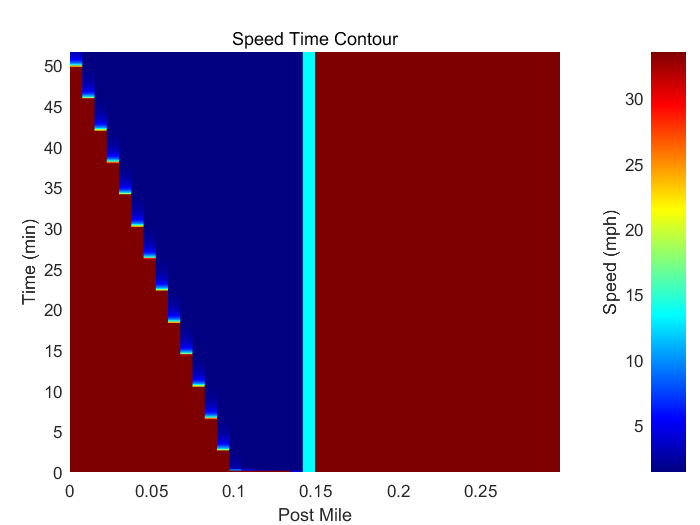
\includegraphics[width=4.00in]{13001400.png}
  \caption{上游流量为1400pcu/h通行能力为1300pcu/h}
\end{figure}
\begin{figure}[H]
  \centering
  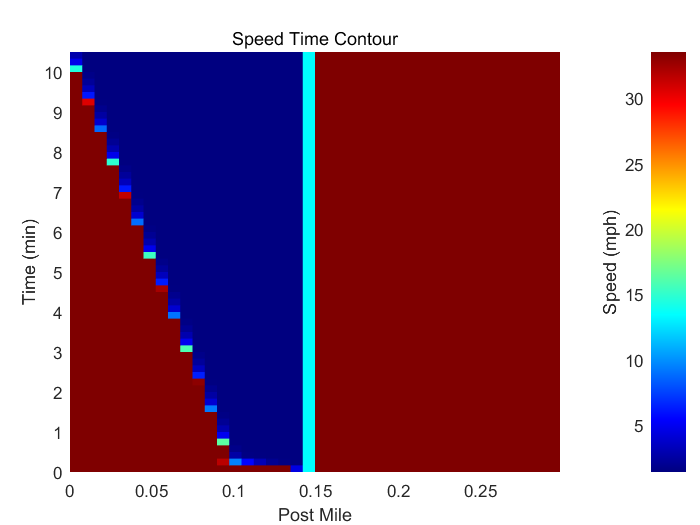
\includegraphics[width=4.00in]{13001800.png}
  \caption{上游流量为1800pcu/h通行能力为1300pcu/h}
\end{figure}
\begin{figure}[H]
  \centering
  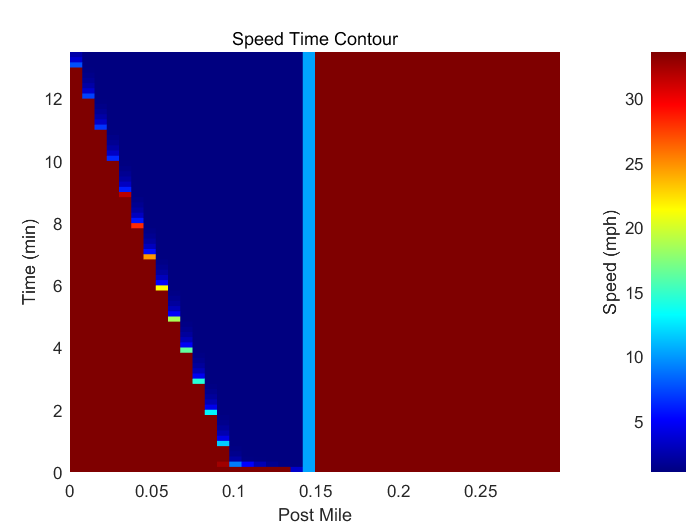
\includegraphics[width=4.00in]{10001400.png}
  \caption{上游流量为1400pcu/h通行能力为1000pcu/h}
\end{figure}
\begin{figure}[H]
  \centering
  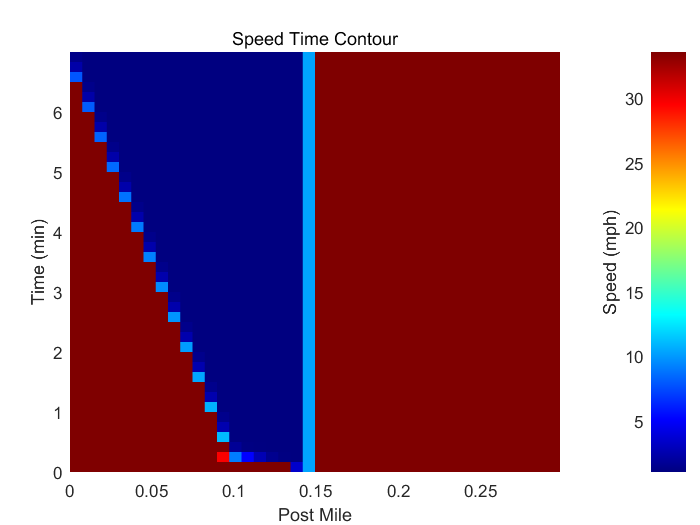
\includegraphics[width=4.00in]{10001800.png}
  \caption{上游流量为1800pcu/h通行能力为1000pcu/h}
\end{figure}
\par由图可知,当上游车流量大于事故路段的通行能力时,到达车流在事故地点会陆续减慢速度甚至停车而集结成密度较高的队列。密度的分界面会沿着车流向后传播,由车流波动理论\cite{par}可知,波速公式为:
$$\omega=\frac{Q_{x}-Q_{y}}{\rho_{x}-\rho_{y}}$$
\par式中:$\omega$——集散波波速;
\par $Q_{x}$、$Q_{y}$——前后两种车流状态的流量;
\par $\rho_{x}$、$\rho_{y}$——前后两种车流状态密度。
\par根据交通流模型可知,交通量Q、行车速度v,车流密度$\rho$三者的关系为:
$$Q=v\times\rho$$
\par 1993年,格林希尔茨(Green-shields)提出了速度-密度线性关系模型:
$$v=v_{f}(1-\rho/\rho_{j})$$
\par式中$v_{f}$——自由流速度;
\par$\rho_{j}$——阻塞密度,即车流密集到所有车辆无法移动时的密度。
\par根据上面的式子,可以推导出波速与密度的关系:
$$\omega=v_{f}(1-\frac{K_{x}+K_{y}}{K_{j}})$$
得到排队长度的计算公式为:
$$L_{j}=\omega\times t= v_{f}(1-\frac{K_{x}+K_{y}}{K_{j}})\times t$$
\section{\heiti\zihao{4}问题四的分析解答}
\subsection{问题分析}
问题一要求我们在视频1(附件1)中的交通事故所处的横断面距离上游路口为140m,路段下游需求不变,上游车流量为1500pcu/h,事故发生时车辆初始排队长度为零,且事故持续不撤离的条件下,估算从事故发生开始,经过多长时间,车辆排队长度到达上游路口。
\par根据问题三的得到的排队长度和上游车流量以及事故断面通行能力的关系,我们将问题四 的参数代入仿真模型中,分析小区路口以及交通灯相位对排队长度的影响。

\subsection{模型的建立和求解}
\subsubsection{在不考虑小区路口和交通灯相位的影响}
道路模型和问题三的相同。用MATLAB对参数进行仿真,得到速度时空分布图如下。
\begin{figure}[H]
  \centering
  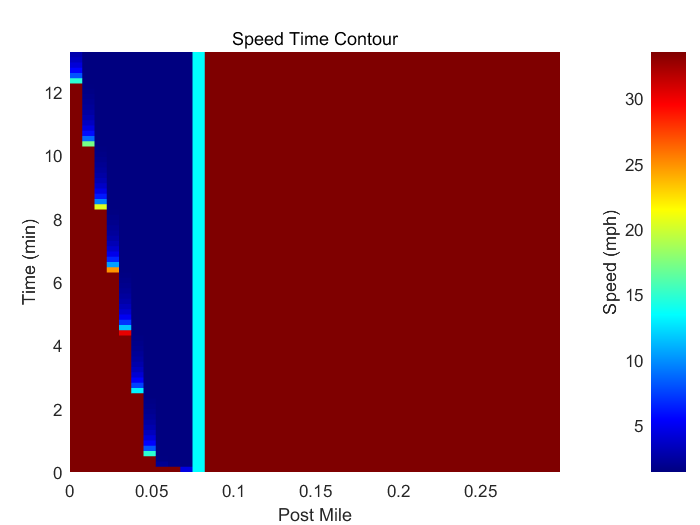
\includegraphics[width=4.00in]{13001500.png}
  \caption{上游车流为1500pcu/h断面通行能力为1300pcu/h时时空分布图}
\end{figure}
\par根据仿真结果可知,事故发生的12分钟后车辆的排队长度会到达上游路口。
\subsubsection{考虑小区路口和交通灯变化的影响}
为了观察小区路口和交通灯信号变化的影响,对采用德国 PTV 公司的交通微观仿真软件VISSIM进行仿真。
\paragraph{仿真参数设定}
不妨假设进入小区的车辆比例为0.1,从小区出来的车流量为100pcu/h。交通灯的相位时间都是30s。
为了尽可能接近现实中事故的影响,在事故路段设立减速区,减速区内速度为15km/h。大型车辆比例为8$\%$仿真模型如下。
\begin{figure}[H]
  \centering
  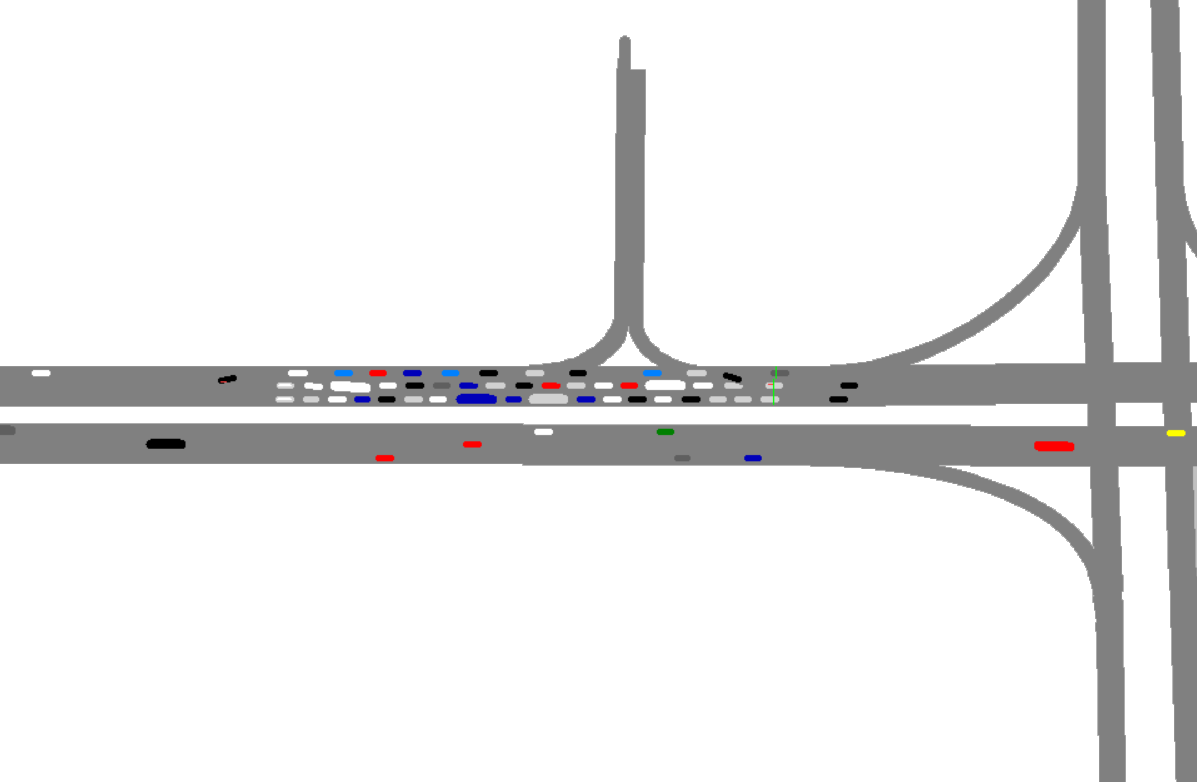
\includegraphics[width=4.00in]{fangzhe.png}
  \caption{vissim仿真模型}
\end{figure}
\par多次仿真对结果取平均值(仿真结果见附录),可得在考虑交通灯和小区路口的影响下,排队车辆到达上游路口的时间为10分钟。
\section{模型的优势和不足}
\subsection{模型的优势}
以交通流特性作为主要研究对象,建立了考虑连续流宏观特性的元胞自动机交通流模型,同时考虑微观和宏观两方面的内容,仿真得到事故发生后路段的时空图,使得结果贴近实际。
\subsection{模型的不足}
针对问题一的模型是基于连续交通流而言的,但是视频中显示的路段为城市道路,多以间歇流为主,交通状况很少能够满足连续流的要求。另外元胞自动机模型是一种通过设定规则,进而模拟交通流的模型,但是规则的设定是否合理,以及设定规则时需要采集多大的样本量,这是可以改进的地方之一。元胞自动机并没有考虑不同车辆类型,如小轿车,大货车,客车等车辆速度特性的影响;很多参数都是通过主观估算确定的,导致结果会有一定的误差
\newpage
\bibliography{mylib}
\newpage
\appendix
\section{vissim仿真结果}
\begin{figure}[H]
  \centering
  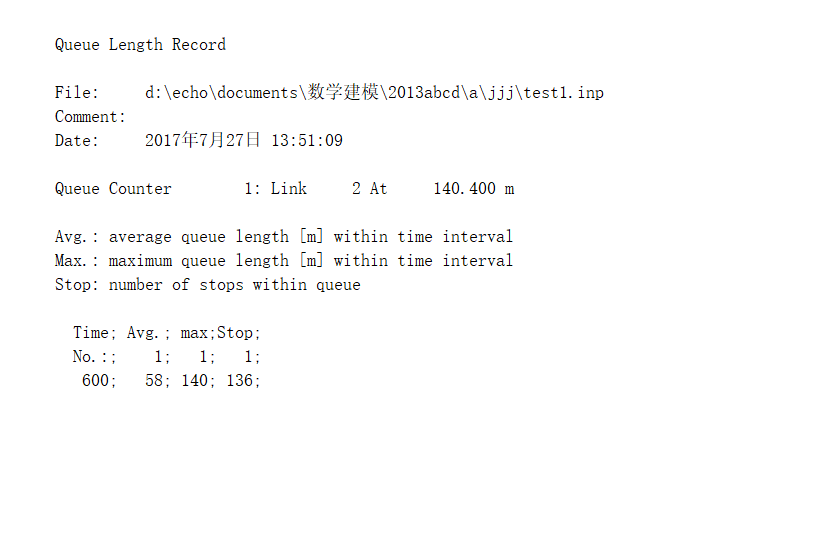
\includegraphics[width=4.00in]{vissim.png}
  \caption{vissim仿真结果}
\end{figure}
\section{matlab代码}
\begin{lstlisting}
function ctmsim(cfg_file, btch)
function ctmsim(cfg_file, btch)
 CTMSIM - starts CTM simulation application.

 Call:
       ctmsim
       ctmsim cfg_file
       ctmsim cfg_file 1

 Parameters:
             cfg_file - .mat configuration file that contains freeway cell data
                         and, possibly, other CTM simulation parameters.
                         This argument is optional, default config file is 'ctm.mat'.
             1        - indicates that CTMSIM should work in the batch mode.
                        This argument is optional.

 Returns:   none.


 Config file must contain 'celldata' variable - it is an array of freeway
 data structures with the following fields:
    cell.PMstart         double (>= 0)            post mile at cell start;
    cell.PMend           double (>= 0)            post mile at cell end;
         Remark: if PMstart <= PMend, the flow goes from left to right,
                 otherwise - from right to left;
    cell.lanes           double (>= 0)            number of lanes;
         Remark: number of lanes may be fractional - auxiliary lanes often
                 are not counted as full lanes;
    cell.FDfmax          double (>= 0)            maximal flow (vph);
    cell.FDrhocrit       double (>= 0)            critical density (vpm);
    cell.FDrhojam        double (>= FDrhocrit)    jam density (vpm);
         Remark: all three fundamental diagram parameters are considered
                 to be total and NOT(!) per lane;
    cell.ORname          char                     on-ramp name;
         Remark: if the cell has no on-ramp, then ORname = [];
    cell.ORlanes         double (>= 0)            number of on-ramp lanes;
    cell.ORflow          double (>= 0)            on-ramp flow (vph);
    cell.ORfmax          double (>= 0)            on-ramp capacity (vph);
         Remark: considered to be total and NOT (!) per lane;
    cell.ORqsize         double (>= 0)            maximum on-ramp queue size;
    cell.ORgamma         double (>= 0 and <= 1)   on-ramp flow blending coefficient (default = 1);
    cell.ORxi            double (>= 0 and <= 1)   on-ramp flow allocation parameter (default = 1);
    cell.ORknob          double (>= 0)            coefficient that adjusts on-ramp demand;
    cell.ORmlcontroller  struct                   on-ramp main line controller structure;
    cell.ORqcontroller   struct                   on-ramp queue controller structure;
    cell.FRname          char                     off-ramp name;
         Remark: if the cell has no off-ramp, then FRname = [];
    cell.FRlanes         double (>= 0)            number of off-ramp lanes;
    cell.FRbeta          double (>= 0 and <= 1)   off-ramp split ratio;
    cell.FRfmax          double (>= 0)            off-ramp capacity (vph);
         Remark: considered to be total and NOT (!) per lane.
    cell.FRknob          double (>= 0)            coefficient that adjusts off-ramp flow;

 Config file may contain other (optional) variables:
 freeway           char                     string that contains freeway name;
 TS                double (>= 0)            sampling period, must be no greater than
                                            min[(cell length)/(free-flow speed)];
 plotTS            double (>= 0)            how often the plots should refresh,
                                            between two plots;
                                            must be greater or equal than TS;
 initiaDensities   double (>= 0)            vector of initial densities, must be
                                            of the same size as number of cells;
 inflow            double (>= 0)            flow that enters given freeway
                                            section (vph);
 outflow           double (>= 0)            flow that is allowed to leave given
                                            freeway section (vph);
 ifKnob            double (>= 0)            coefficient that adjusts mainline demand;
 ofKnob            double (>= 0)            coefficient that adjusts capacity downstream of the last cell;
 timeout           double (>= 0)            how many seconds to wait between
                                            two plots;
 taxislim          double (>= 0)            limit for time axis in time series plots
                                            measured in plotted time steps;
 densityCMF        double (1024 x 3)        color map for time series density contour;
 flowCMF           double (1024 x 3)        color map for time series flow contour;
 orflowCMF         double (1024 x 3)        color map for time series on-ramp flow contour;
 orqueueCMF        double (1024 x 3)        color map for time series on-ramp queue contour;
 frflowCMF         double (1024 x 3)        color map for time series off-ramp flow contour;
 frbetaCMF         double (1024 x 3)        color map for time series off-ramp split ratio contour;
 speedCMF          double (1024 x 3)        color map for time series speed contour;
 vhtCMF            double (1024 x 3)        color map for time series VHT contour;
 vmtCMF            double (1024 x 3)        color map for time series VMT contour;
    Remark: for information on default color maps, type 'help graph3d';
 yoColorRatio      double (>= 0 and <= 1)   array of two numbers that indicate
                                            fractions of maximum flow the flow must
                                            achieve in free flow or congested mode
                                            to make cell color yellow or orange;
 demandProfile     double (>= 0)            array of on-ramp demand values whose size is
                                            (number of cells + 2) x (number of time samples);
 demandTS          double (>= 0)            sampling time for the demand in demandProfile,
                                            must be greater or equal than TS;
 betaProfile       double (>= 0 and <= 1)   array of off-ramp split ratios whose size is
                                            (number of cells) x (number of time samples);
 betaTS            double (>= 0)            sampling time for the split ratio in betaProfile,
                                            must be greater or equal than TS;
 frflowProfile     double (>= 0 and <= 1)   array of off-ramp flow values whose size is
                                            (number of cells) x (number of time samples);
 frflowTS          double (>= 0)            sampling time for the flow in frflowProfile,
                                            must be greater or equal than TS;
 maxSimStep        double (>= 0)            maximum simulation step;
 maxSimTime        double (>= 0)            maximum simulation time:
                                               number_of_steps * TS;
 dataFile          char                     string with a file name where the
                                            simulation data is to be saved;
    Remark: last three parameters make difference only in the batch mode.


 See also:   FWCONFIG, PLOTSIM.

 Last modified:   03/18/2007.


 Alex Kurzhanskiy   <akurzhan@eecs.berkeley.edu>

global g_ctmGUI;
if nargin & isa(cfg_file, 'char')
  g_ctmGUI.configFile = cfg_file;
end
if nargin < 2
  ctmGUI;
else
  ctmBATCH;
end
return;

\end{lstlisting}
\end{document} 